\documentclass[compress]{beamer}

\usepackage{multicol}
\usepackage{cite}

% \usepackage{beamerthemesplit}   %Activate for custom appearance
%\usetheme{Copenhagen}
%\usecolortheme{seahorse}

%\usepackage{beamerouterthemetwolines}

\usetheme{Madrid}
\useoutertheme[subsection=false]{miniframes} % Alternatively: miniframes, infolines, split
\useinnertheme{circles}
\definecolor{UBCblue}{rgb}{0.09, 0.21, 0.25} % UBC Blue (primary)
\usecolortheme[named=UBCblue]{structure}


\newcommand*{\Scale}[2][4]{\scalebox{#1}{$#2$}}%
\newcommand*{\Resize}[2]{\resizebox{#1}{!}{$#2$}}%

\usepackage{tikz}
\usetikzlibrary{shapes,arrows}
\tikzstyle{line}=[draw]
\tikzstyle{startstop} = [rectangle, rounded corners, minimum width=3cm, minimum height=1cm,text centered, draw=black, fill=red!30]
\tikzstyle{io} = [trapezium, trapezium left angle=70, trapezium right angle=110, minimum width=3cm, minimum height=1cm, text centered, draw=black, fill=blue!30]
\tikzstyle{process} = [rectangle, minimum width=3cm, minimum height=1cm, text centered, draw=black, fill=orange!30]

\tikzstyle{phage} = [rectangle, minimum width=3cm, minimum height=1cm, text centered, draw=black, fill=orange!30]
\tikzstyle{bacteria} = [rectangle, minimum width=3cm, minimum height=1cm, text centered, draw=black, fill=blue!30]
\tikzstyle{resource} = [rectangle, minimum width=3cm, minimum height=1cm, text centered, draw=black, fill=green!30]
\tikzstyle{G} = [rectangle,rounded corners,minimum width=3cm, minimum height=1cm, text centered, draw=white, fill=gray!30]

\tikzstyle{bnode} = [circle, minimum width=1cm, minimum height=1cm, text centered, draw=black, fill=blue!30]
\tikzstyle{pnode} = [octagon, minimum width=1cm, minimum height=1cm, text centered, draw=black, fill=red!30]

\tikzstyle{decision} = [diamond, minimum width=3cm, minimum height=1cm, text centered, draw=black, fill=green!30]
\tikzstyle{arrow} = [thick,->,>=stealth]
\tikzstyle{arrowb} = [thick,<->,>=stealth]
\tikzstyle{arrowNo} = [thick,-|,>=stealth]
\usetikzlibrary{positioning,calc,arrows}
\usetikzlibrary{shapes,snakes}

\newenvironment{nonavig}
{\begingroup
	\renewcommand*\insertshorttitle{}
	\renewcommand*\insertshortauthor{}
	\renewcommand*\insertshortinstitute{}
	\renewcommand*\dohead{\rule{0em}{1.75em}}}
{\endgroup}

\tikzset{somestyle/.style={draw,circle,fill,fill opacity=0.1}}
\tikzset{somestyle2/.style={draw,ellipse, minimum width=300pt, align=center,fill,fill opacity=0.1}}
\tikzset{somestyle3/.style={draw,ellipse, minimum width=100pt, align=center,fill,fill opacity=0.1}}

%\newcommand{\semitransp}[2][35]{\color{fg!#1}#2}

%\usepackage{lastpage}
\usepackage{textcomp}
\usepackage{booktabs}
\usepackage{array}
\usepackage{xcolor}
\usepackage{multicol}
\usepackage{soul}
\definecolor{olive}{rgb}{0.3, 0.4, .1}
\definecolor{fore}{RGB}{249,242,215}
\definecolor{back}{RGB}{51,51,51}
\definecolor{title}{RGB}{255,0,90}
\definecolor{dgreen}{rgb}{0.,0.6,0.}
\definecolor{gold}{rgb}{1.,0.84,0.}
\definecolor{JungleGreen}{cmyk}{0.99,0,0.52,0}
\definecolor{BlueGreen}{cmyk}{0.85,0,0.33,0}
\definecolor{RawSienna}{cmyk}{0,0.72,1,0.45}
\definecolor{Magenta}{RGB}{238,51,119}
\definecolor{Teal}{RGB}{0,153,136}

\setbeamertemplate{navigation symbols}{}

%Title Slide Info
\title[MK Test]{The McDonald-Kreitman Test For Selection: An Extremely Brief Introduction}
\author[Jake L. Weissman]{Jake L. Weissman}
\date{May 19, 2020}  %%%%% change date
%\institute{University of Maryland, College Park}

\newcommand{\semitransp}[2][35]{\textcolor{fg!#1}{#2}}

\usepackage[authoryear]{natbib}
%\setbeamercovered{transparent} 
%Begin Document

\usepackage[percent]{overpic}
\usepackage{contour}

\logo{%
  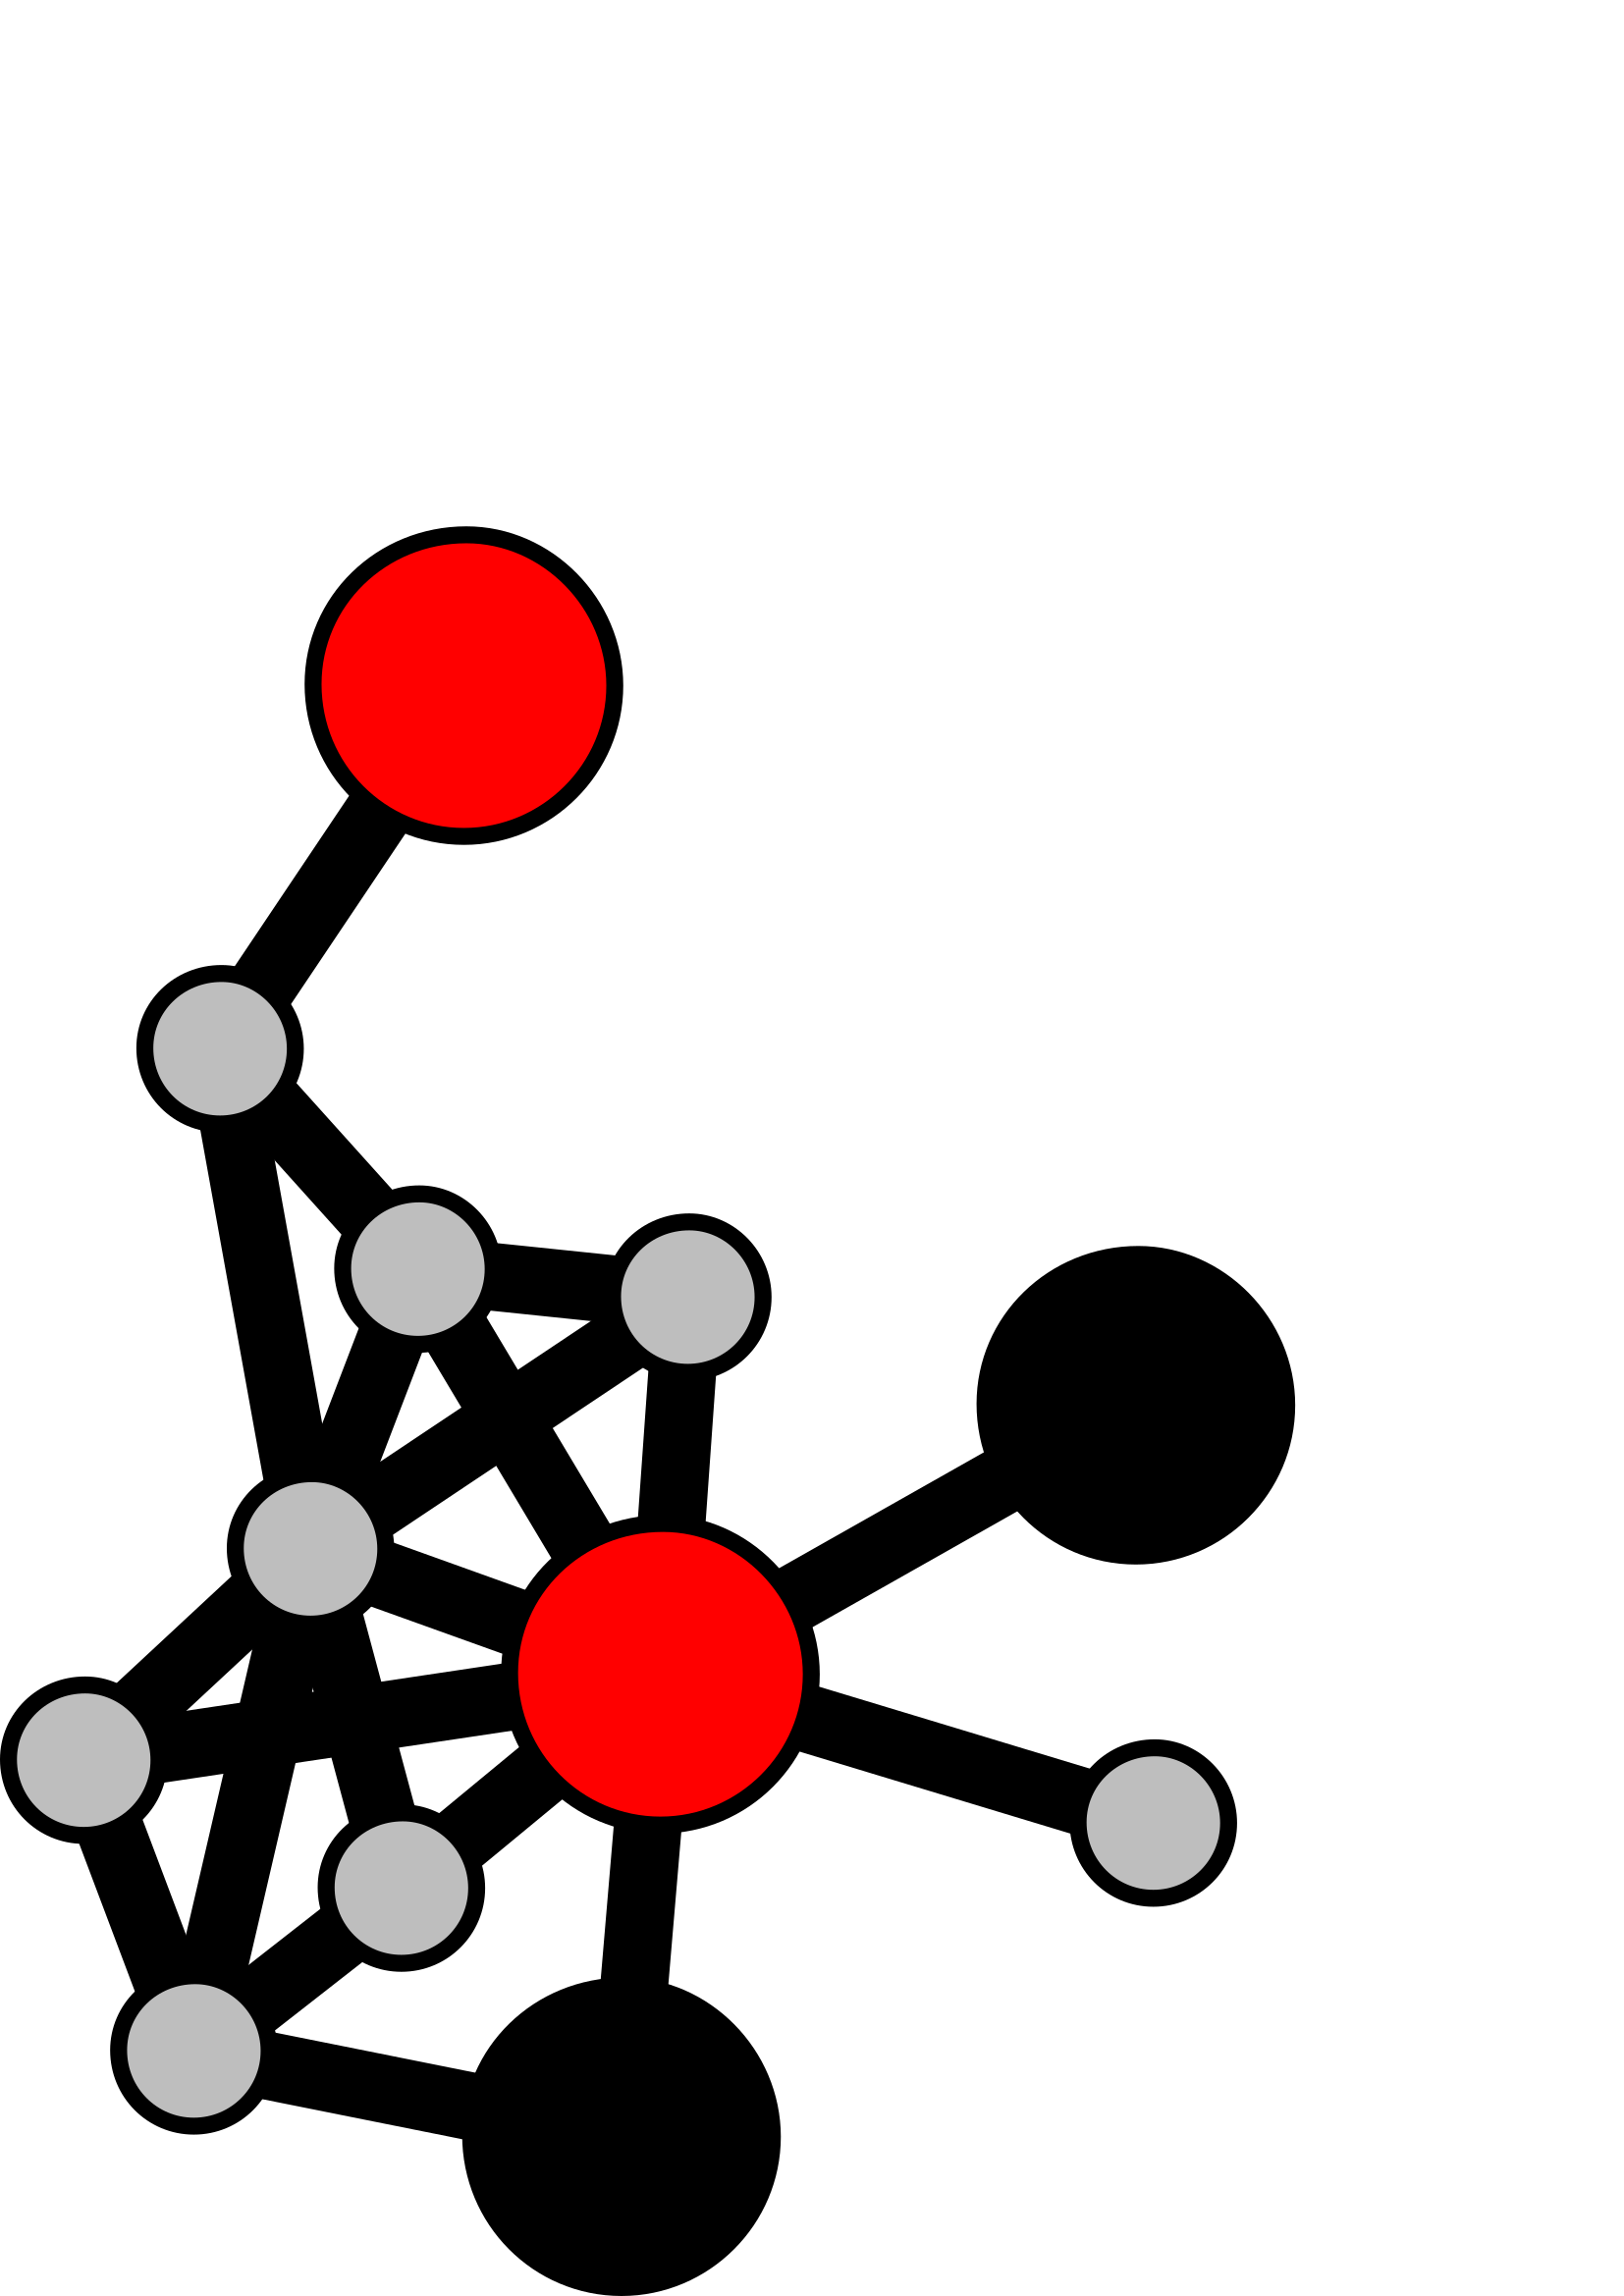
\includegraphics[scale=.1]{LOGO.png}
   }

\begin{document}
\contourlength{2pt} %how thick each copy is
\contournumber{20}  
%%%%%
% Title %
%%%%%R

\begin{frame}
\maketitle
\end{frame}

\begin{frame}{Last Time: $dN/dS$}
\begin{itemize}
\item Only needs divergence data 
\item Unlikely to be $>1$ (indicating positive seln) except in extreme cases, not particularly sensitive
\end{itemize}
\end{frame}


\begin{frame}{This Time: MK-Test}
\begin{itemize}
\item Needs polymorphism and substitution data
\item Much more likely to pick up positive selection
\end{itemize}
\end{frame}

\begin{frame}{Intuition}
\begin{itemize}
\item Polymorphism is \emph{recent}
\begin{itemize}
\item Selection hasn't had time to act
\item Strongly positively selected alleles fix so rapidly that you don't see them among polymorphisms
\end{itemize}
\item Therefore polymorphism will not show effects of selection, but substitutions will
\item The MK Test compares the fraction of nonsynonymous differences looking at polymorphisms and substitutions respectively, taking polymorphism as the null distribution of nonsynonymous differences (without selection)
\end{itemize}
\end{frame}

\begin{frame}{Quantities}
The MK-test requires you to calculate four quantities:
\begin{itemize}
\item $P_N$: Number of nonsynonymous polymorphisms
\item $P_S$: Number of synonymous polymorphisms
\item $D_N$: Number of nonynonymous fixed difference
\item $D_S$: Number of synonymous fixed differences

\begin{table}[]
\begin{tabular}{lllll}
\cline{2-3}
\multicolumn{1}{l|}{}               & \multicolumn{1}{l|}{Fixed} & \multicolumn{1}{l|}{Polymorphic} &  &  \\ \cline{1-3}
\multicolumn{1}{|l|}{Synonymous}    & \multicolumn{1}{l|}{$D_S$}         & \multicolumn{1}{l|}{$P_S$}         &  &  \\ \cline{1-3}
\multicolumn{1}{|l|}{Nonsynonymous} & \multicolumn{1}{l|}{$D_N$}         & \multicolumn{1}{l|}{$P_N$}         &  &  \\ \cline{1-3}
                                    &                                    &                                    &  & 
\end{tabular}
\end{table}
\end{itemize}
\end{frame}

\begin{frame}{Typical Data}
\begin{itemize}
\item 2+ sequences of your gene of interest from your population of interest (to assess polymorphism)
\item One (or sometimes more) sequence from an outgroup (to assess fixed differences)
\end{itemize}
\end{frame}

\begin{frame}{The Test}
\centering
$$H_0: \frac{P_N}{P_S} \approx \frac{D_N}{D_S}$$
\begin{table}[]
\begin{tabular}{lllll}
\cline{2-3}
\multicolumn{1}{l|}{}               & \multicolumn{1}{l|}{Fixed} & \multicolumn{1}{l|}{Polymorphic} &  &  \\ \cline{1-3}
\multicolumn{1}{|l|}{Synonymous}    & \multicolumn{1}{l|}{$D_S$}         & \multicolumn{1}{l|}{$P_S$}         &  &  \\ \cline{1-3}
\multicolumn{1}{|l|}{Nonsynonymous} & \multicolumn{1}{l|}{$D_N$}         & \multicolumn{1}{l|}{$P_N$}         &  &  \\ \cline{1-3}
                                    &                                    &                                    &  & 
\end{tabular}
\end{table}


{\bf Test for independence:}
\begin{itemize}
\item Fisher's Exact Test (little data)
\item $\chi^2$ (lots of data)
\end{itemize}
\end{frame}

\begin{frame}{Extensions}

{\bf MK-test will often fail to detect positive selection in the presence of weak purifying selection}
\begin{itemize}
\item Several methodological approaches to correct for this (implemented in iMKT package we will use for interactive lesson portion)
\item The simplest approach is to just remove low-frequency polymorphisms, since these are more likely to be under weak purifying selection (Fay, Wyckoff and Wu, 2001)
\end{itemize}

\end{frame}

\begin{frame}{Neutrality Index}
$$\text{NI} = \frac{\left( \frac{P_N}{D_N} \right)}{\left( \frac{P_S}{D_S} \right)}$$
\begin{itemize}
\item Useful for when you want to compare degree of selection across genes
\end{itemize}
\end{frame}

\begin{frame}{Alpha}
$$\alpha = 1 - \frac{D_S P_N}{D_N P_S} = 1-\text{NI}$$
\begin{itemize}
\item Proportion of nonsynonymous substitutions fixed by positive selection (but see Stoletzki and Eyre-Walker, 2011. ``Estimation of the neutrality index.'' \emph{MBE})
\end{itemize}
\end{frame}

\end{document}